\begin{mainquestion}{diode_hogging}{Parallel Diodes}
We explore the case of two identical diodes placed in parallel as shown in the accompanying figure. Assume the diodes have $n = 1$. For each diode, a forward current of \qty{200}{\milli\ampere} results in a voltage of \qty{900}{\milli\volt} at \qty{300}{\kelvin}.

\begin{center}
    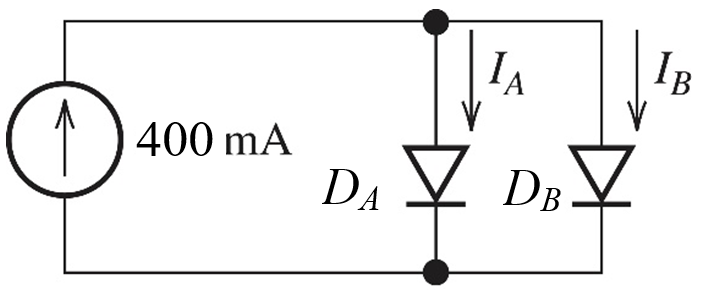
\includegraphics[width=0.5\textwidth]{questionbank/diodes/diode_hogging/v0/diode_schematic.png}
\end{center}

% =========================================================
\begin{partquestion}{current}
{If both diodes are at 300 K, what are the values of $I_A$ and $I_B$?}

\begin{answer}
Using KCL, $I_A + I_B = \qty{400}{\milli\ampere}$. Since the diodes are identical, by symmetry we expect $I_A = I_B = \qty{200}{\milli\ampere}$.
\end{answer}
\end{partquestion}

% =========================================================
\begin{partquestion}{currenthot}
{If diode A is at 300 K and diode B is at 310 K, find $I_A$ and $I_B$ using the rule of thumb that $I_S$ doubles every 5 K increase in temperature.}

\begin{answer}
We first determine $I_S$ at 300 K by plugging in known values of operation:
\[
I_S
=
I \exp\!\left(-\frac{qV_{DA}}{nkT}\right)
=
\left(\qty{200}{\milli\ampere}\right)
\exp\!\left(-\frac{1.6\times10^{-19}\cdot0.900}{1\cdot1.38\times10^{-23}\cdot300}\right)
=
1.56\times10^{-16}\,\mathrm{A}
\]

Now we can find the diode currents:
\[
\qty{0.4}{\ampere}
=
I_A + I_B
=
I_S \exp\!\left(38.63 V_{DA}\right)
+
4 I_S \exp\!\left(37.38 V_{DB}\right)
\]

Note the factor of 4 in the second term arises because when temperature increases by 10 K, $I_S$ quadruples. This is a transcendental equation that can be solved numerically using MATLAB, Newton’s method, or trial and error and results in $V_D = \qty{0.896}{\volt}$.

It follows using
\[
I \approx I_S \exp\!\left(\frac{V_{D}}{nV_T}\right)
\]
that $I_A = \qty{0.173}{\ampere}$ and $I_B = \qty{0.227}{\ampere}$.
\end{answer}
\end{partquestion}

% =========================================================
\begin{partquestion}{heat}
{Based on your result from (b), which diode will heat up, and which will cool down?}

\begin{answer}
Diode $D_B$, with an increase in current (from \qty{0.2}{\ampere} to \qty{0.227}{\ampere}), will experience an increase in temperature. Diode $D_A$, with a decrease in current (from \qty{0.2}{\ampere} to \qty{0.173}{\ampere}), will experience a decrease in temperature.
\end{answer}
\end{partquestion}

% =========================================================
\begin{partquestion}{hogging}
{What will happen to the diodes as their temperatures change? Describe the potential problem.}

\begin{answer}
As diode $D_B$ continues to heat up, we know its current will continue to increase as well—a bit of undesired positive feedback. Over a short period of time, this can lead to “current hogging” and cause diode $D_B$ to conduct nearly all of the current, while diode $D_A$ sits relatively idle. Situations like this are undesirable because it is often easy to exceed the rated specifications and cause damage to a device if it is carrying more current than intended.
\end{answer}
\end{partquestion}

% =========================================================
\begin{partquestion}{solver}
{One possible mitigation for the problem discussed in (d) is the addition of a series resistor $R$ in series with each diode. Find an expression for $R$ in terms of the currents $I_A$ and $I_B$ and the voltages $V_{DA}$ and $V_{DB}$.}

\begin{center}
    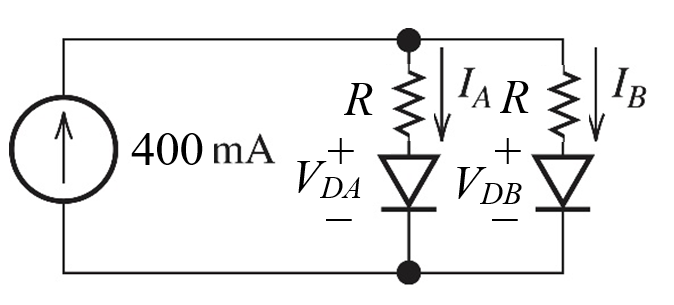
\includegraphics[width=0.5\textwidth]{questionbank/diodes/diode_hogging/v0/diode_rs_schematic.png}
\end{center}

\begin{answer}
Assuming a voltage $V$ across the current source, we can use Ohm’s law:
\[
I_A = \frac{V - V_{DA}}{R}
\qquad
I_B = \frac{V - V_{DB}}{R}
\]

Eliminating $V$ gives:
\[
I_A R + V_{DA} = I_B R + V_{DB}
\]

so
\[
R = \frac{V_{DB} - V_{DA}}{I_A - I_B}.
\]
\end{answer}
\end{partquestion}

% =========================================================
\begin{partquestion}{findr}
{Find the value for $R$ that ensures the currents $I_A$ and $I_B$ are within 1\% of one another, assuming the temperatures remain as they were in part (b).}

\begin{answer}
We have $I = I_A + I_B$ and the constraint $I_A \ge 0.99 I_B$. (Since $D_A$ is cooler than $D_B$, we expect an inherent upper bound of the current where $I_A\le I_B$.)  This implies $I_B \le \frac{I}{1.99}$, giving $I_B \le \qty{0.201}{\ampere}$ and thus $I_A \ge \qty{0.199}{\ampere}$.

At equality:
\[
V_{DA} = \frac{nkT_1}{q}\ln\!\frac{I_A}{I_S}
\qquad
V_{DB} = \frac{nkT_2}{q}\ln\!\frac{I_B}{4I_S}
\]

where $T_1 = \qty{300}{\kelvin}$ and $T_2 = \qty{310}{\kelvin}$.

Plugging in all the known values gives $V_{DA} = \qty{0.900}{\volt}$ and $V_{DB} = \qty{0.893}{\volt}$. Then
\[
R = \frac{V_{DB} - V_{DA}}{I_A - I_B}
=
\frac{0.900 - 0.893}{0.199 - 0.201}
=
\qty{3.38}{\ohm}.
\]

\end{answer}
\end{partquestion}

% =========================================================
\begin{partquestion}{voltage}
{Calculate the voltage across the current source.}

\begin{answer}
Using $I_A = \frac{V - V_{DA}}{R}$:
\[
V = I_A R + V_{DA}
= (0.199)(3.38) + 0.9000
= \qty{1.57}{\volt}.
\]

(We could have used the equivalent expression with $I_B$ and obtained the same result.)
\end{answer}
\end{partquestion}

% =========================================================
\begin{partquestion}{power}
{What is the ratio of the dissipated power in the two resistors to that of the remaining dissipated power?}

\begin{answer}
The total dissipated power is equal to the total supplied power
\[
VI = (1.57)(0.4) = \qty{0.629}{\watt}.
\]
The total power dissipated in the resistors (about 43\%) is
\[
I_A^2 R + I_B^2 R
=
(0.199)^2(3.38) + (0.201)^2(3.38)
=
\qty{0.271}{\watt}.
\]
and the remaining dissipated power must be 
\[
0.629 - 0.271 = \qty{0.358}{\watt}.
\]
all of which are consumed by the two diodes. The desired ratio is:
\[
\frac{0.271}{0.358} \approx 0.75.
\]
\end{answer}
\end{partquestion}

\end{mainquestion}